\documentclass[11pt]{article}
\usepackage{hyperref}
\usepackage[english]{babel}
\usepackage{blindtext}
\usepackage{url}
\usepackage{graphicx}
\usepackage{multicol}
\usepackage[center]{titlesec}
\usepackage{geometry}
\usepackage{lettrine} % The lettrine is the first enlarged letter at the beginning of the text

%\usepackage{mathtools}

\usepackage[sort, numbers]{natbib}


%
%\setlength{\columnseprule}{0.4pt}
%\setlength{\footskip}{20pt}
\usepackage{fancyhdr}
\fancyhf{}
\fancyhead[C]{Weather data $\bullet$ Joe Brew }
\fancyfoot[C]{  $\bullet$ Uganda \bullet$  }
\renewcommand\headrulewidth{1pt}
\renewcommand\footrulewidth{1pt}
\pagestyle{fancy}

%

\setlength{\columnsep}{1.5cm}
%\setlength{\columnseprule}{0.4pt}

%\MakeOuterQuote{"}



\graphicspath{ {/home/joebrew/Documents/weather/uganda/uganda_weather_first_pass} }

%the next two lines adjust the third, centered section of the exec sum
\def\changemargin#1#2{\list{}{\rightmargin#2\leftmargin#1}\item[]}
\let\endchangemargin=\endlist 

\usepackage{Sweave}
\begin{document}
\Sconcordance{concordance:uganda_weather_first_pass.tex:uganda_weather_first_pass.Rnw:%
1 42 1 1 0 8 1 1 21 1 3 83 1 1 75 1 2 1 1 1 75 1 2 44 1}


\title{\textbf{Uganda Weather: First Pass}}
\author{Joe Brew}


\maketitle

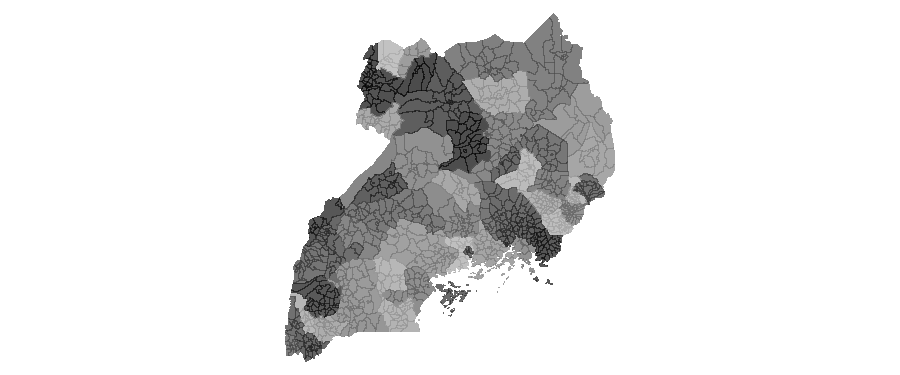
\includegraphics{uganda_weather_first_pass-001}

\emph{
\noindent The following is a brief overview of a first attempt to systematically collect Ugandan weather-related data.  I outline (a) the method employed (webscraping from Wunderground), (b) the results (mediocre at best), (c) advantages (few) and shortcomings (many) and (d) options for moving forward. }
\tableofcontents

\vspace{20mm}

\begin{center}

\includegraphics[width=2cm]{logo}
\end{center}


\newgeometry{margin=2.5cm}
%\fancyhfoffset[E,O]{0pt}


%------------------------------------------
\section*{Webscraping Ugandan weather data}
\addcontentsline{toc}{section}{Webscraping Ugandan weather data}
%------------------------------------------
\hrulefill

\begin{multicols}{2} 
\setkeys{Gin}{width=0.45\textwidth}

%------------------------------------------
\subsection*{Method}
\addcontentsline{toc}{subsection}{Method}
%------------------------------------------

\lettrine[nindent=0em,lines=3]{B}{la} bla bla bla.\cite{Cottler2014} \blindtext 

%------------------------------------------
\subsection*{Results}
\addcontentsline{toc}{subsection}{Results}
%------------------------------------------
\blindtext

\begin{center}
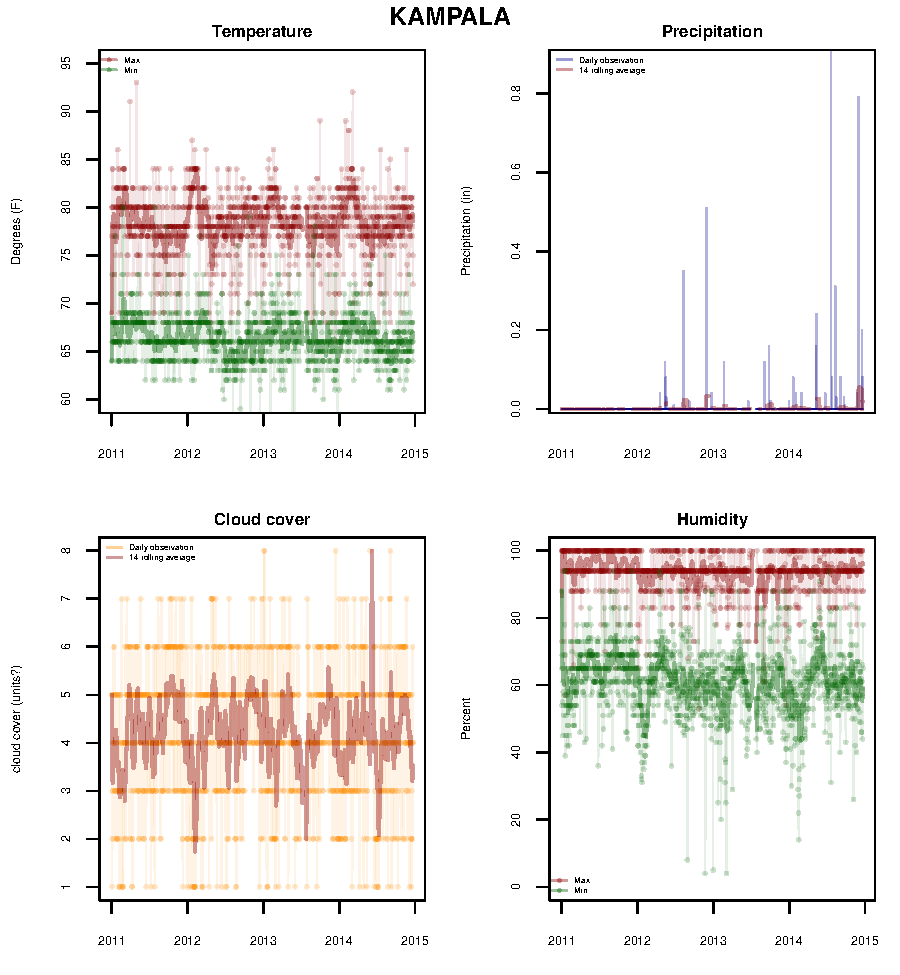
\includegraphics{uganda_weather_first_pass-002}
\end{center}

%------------------------------------------
\subsection*{Advantages and shortcomings}
\addcontentsline{toc}{subsection}{Advantages and shortcomings}
%------------------------------------------
\blindtext

%------------------------------------------
\subsection*{Moving forward}
\addcontentsline{toc}{subsection}{Moving forward}
%------------------------------------------
\blindtext




\end{multicols}
\setkeys{Gin}{width=1\textwidth}
%----------------------------------------------------------------------------------------
%  REFERENCE LIST
%----------------------------------------------------------------------------------------
\newpage
\bibliographystyle{unsrtnat}
\bibliography{bibliography}


\end{document}
